\documentclass[30pt,a3paper,portrait]{tikzposter}
\usepackage[utf8]{inputenc}
\usepackage{xcolor}
\usepackage{graphicx}
\usepackage{multicol}
\usepackage{tikz}
\usepackage{adjustbox}

% Title and author setup
\title{Gait Pattern Recognition
with an Arduino Nano 33 BLE}
\author{Fedor Kotiaev and Abishek Senthilkumar}
\titlegraphic{
    
\includegraphics[height=6.5cm]{images/logo_hs_technik}
    \hfill
    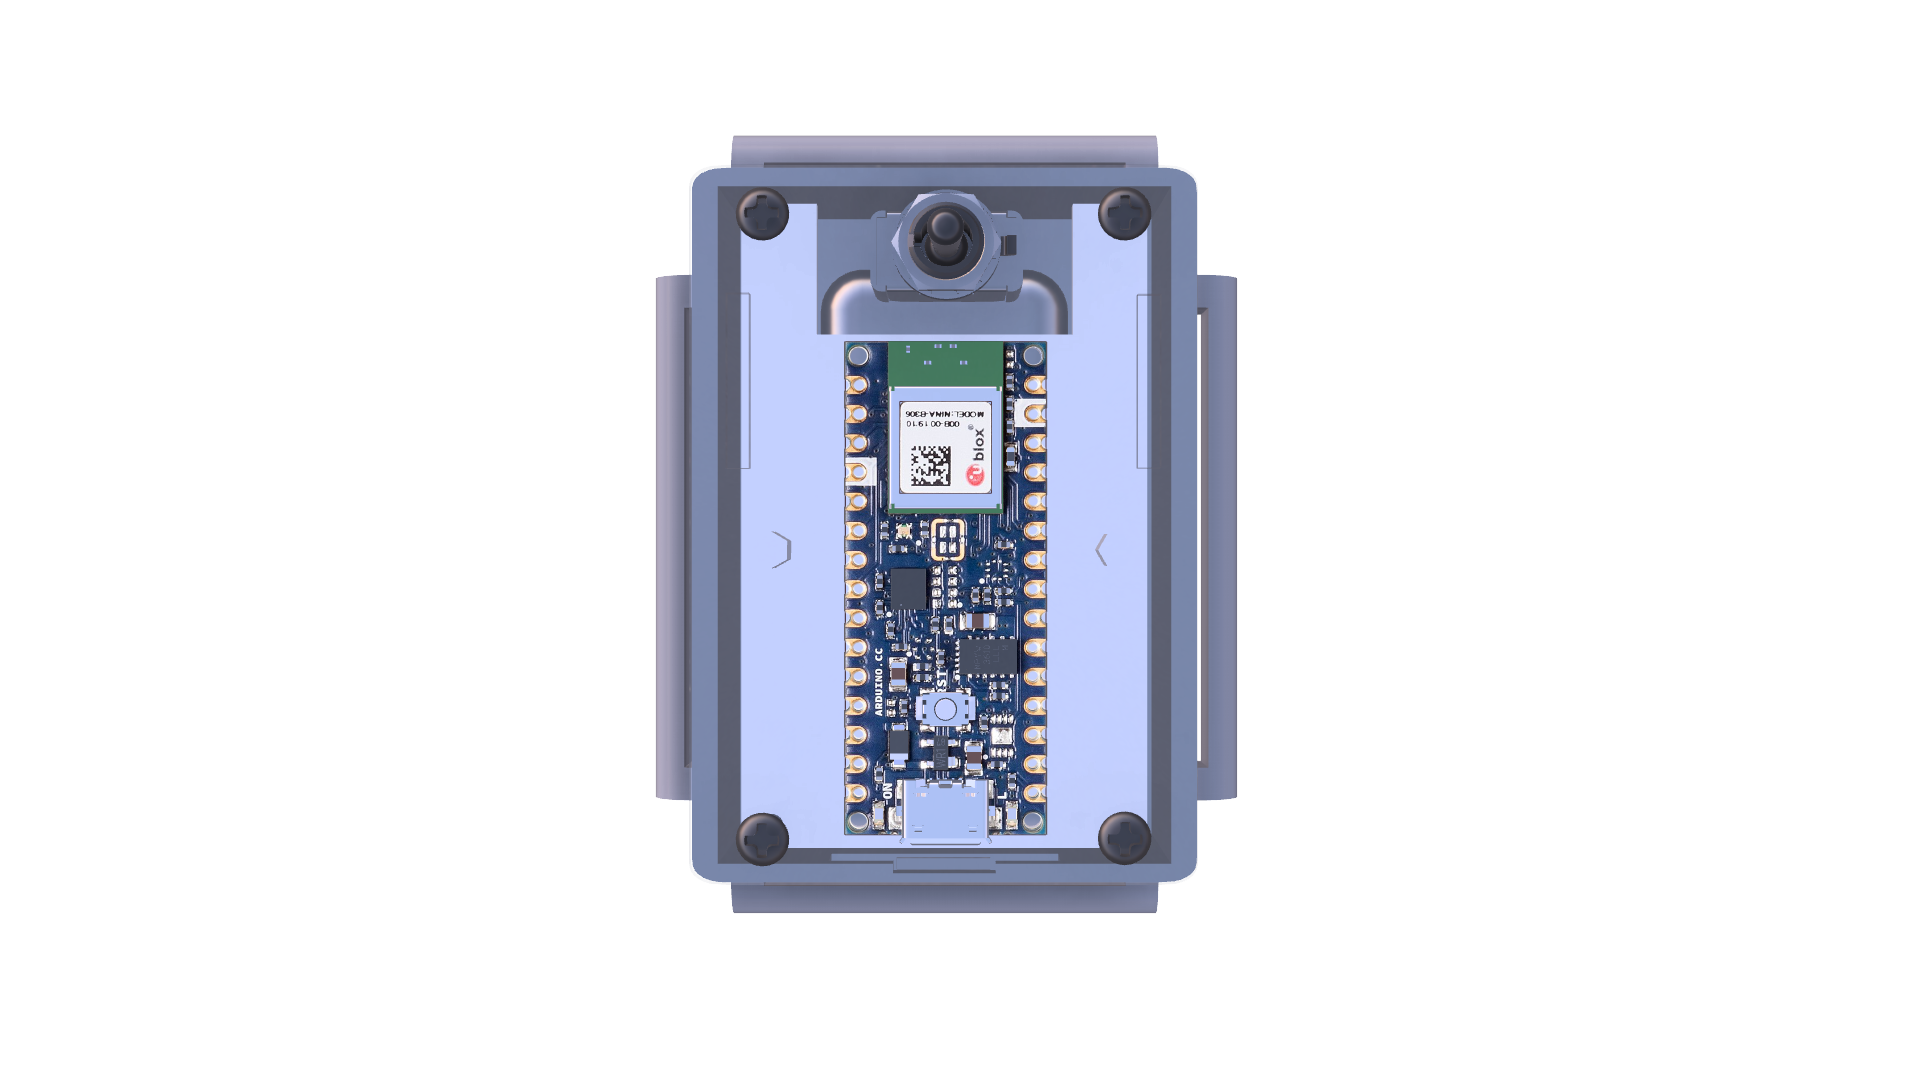
\includegraphics[height=6.5cm]{images/ourlogo}
}

% Poster theme
\usetheme{Desert}

\begin{document}
\maketitle

% Two-column structure starts
\begin{columns}

% Column 1: Content
\column{0.5}
{
    \block{Gait Analysis for Parkinson’s Disease}{
        {\Large
        Wearable devices have revolutionized healthcare by enabling continuous tracking of health parameters and the early detection of diseases. This project follows the motivation to develop a wearable system capable of detecting abnormal gait patterns caused by diseases like Parkinson’s. Early detection can prevent falls, improve outcomes, and provide actionable insights for caregivers and healthcare professionals.

        Gait analysis plays a crucial role in health monitoring. Parkinson’s disease, for example, alters walking by causing shorter steps, shuffling, and instability. Similarly, strokes lead to asymmetric gait and reduced mobility. Motivated by these challenges, we aim to create a device that utilizes this technology to monitor these parameters, enabling early intervention, mitigating risks, and improving patients’ quality of life.
        }
    }

    \block{Technical Challenges}{
        {\Large
        Developing this system posed several challenges:
        \begin{itemize}
            \item \textbf{Sensor Noise:} IMU sensors are sensitive to environmental interference.
            \item \textbf{Real-Time Processing:} Limited computational power of the Arduino Nano 33 BLE Sense.
            \item \textbf{Gait Variability:} Diverse walking patterns influenced by terrain, speed, and physical conditions.
            \item \textbf{Design Constraints:} The device had to be compact, lightweight, and user-friendly while maintaining reliability.
        \end{itemize}
        }
    }

    \block{Solutions and System Design}{
        {\Large
        \begin{itemize}
            \item \textbf{Noise Reduction:} Implemented Kalman filters to enhance sensor accuracy.
            \item \textbf{Machine Learning:} Applied TinyML techniques to adapt models for embedded hardware.
           \item \textbf{Hardware Efficiency:} The device is equipped with a coin cell battery holder that holds two 20mm CR2032 batteries, providing  about 44 hours of continuous operation.
        \end{itemize} 
        \begin{tikzfigure}
            \includegraphics[width=1.1\linewidth]{images/phototitile} % 
        \end{tikzfigure}
        \textbf{Fig. 1:} Assembled prototype of the device.
        }
    }
}

% Column 2: Content
\column{0.5}
{
    \block{System Design}{
        {\Large
        The body case was designed in AutoFusion to:
        \begin{itemize}
            \item Enhance lightweight construction.
            \item Provide wide space for the battery and control elements.
            \item Ensure modularity and easy battery replacement.
            \item Offer good indication through visible LED lights.
        \end{itemize}

        These features make the system practical for daily use, bridging the gap between clinical diagnostics and at-home healthcare.
        \begin{tikzfigure}
            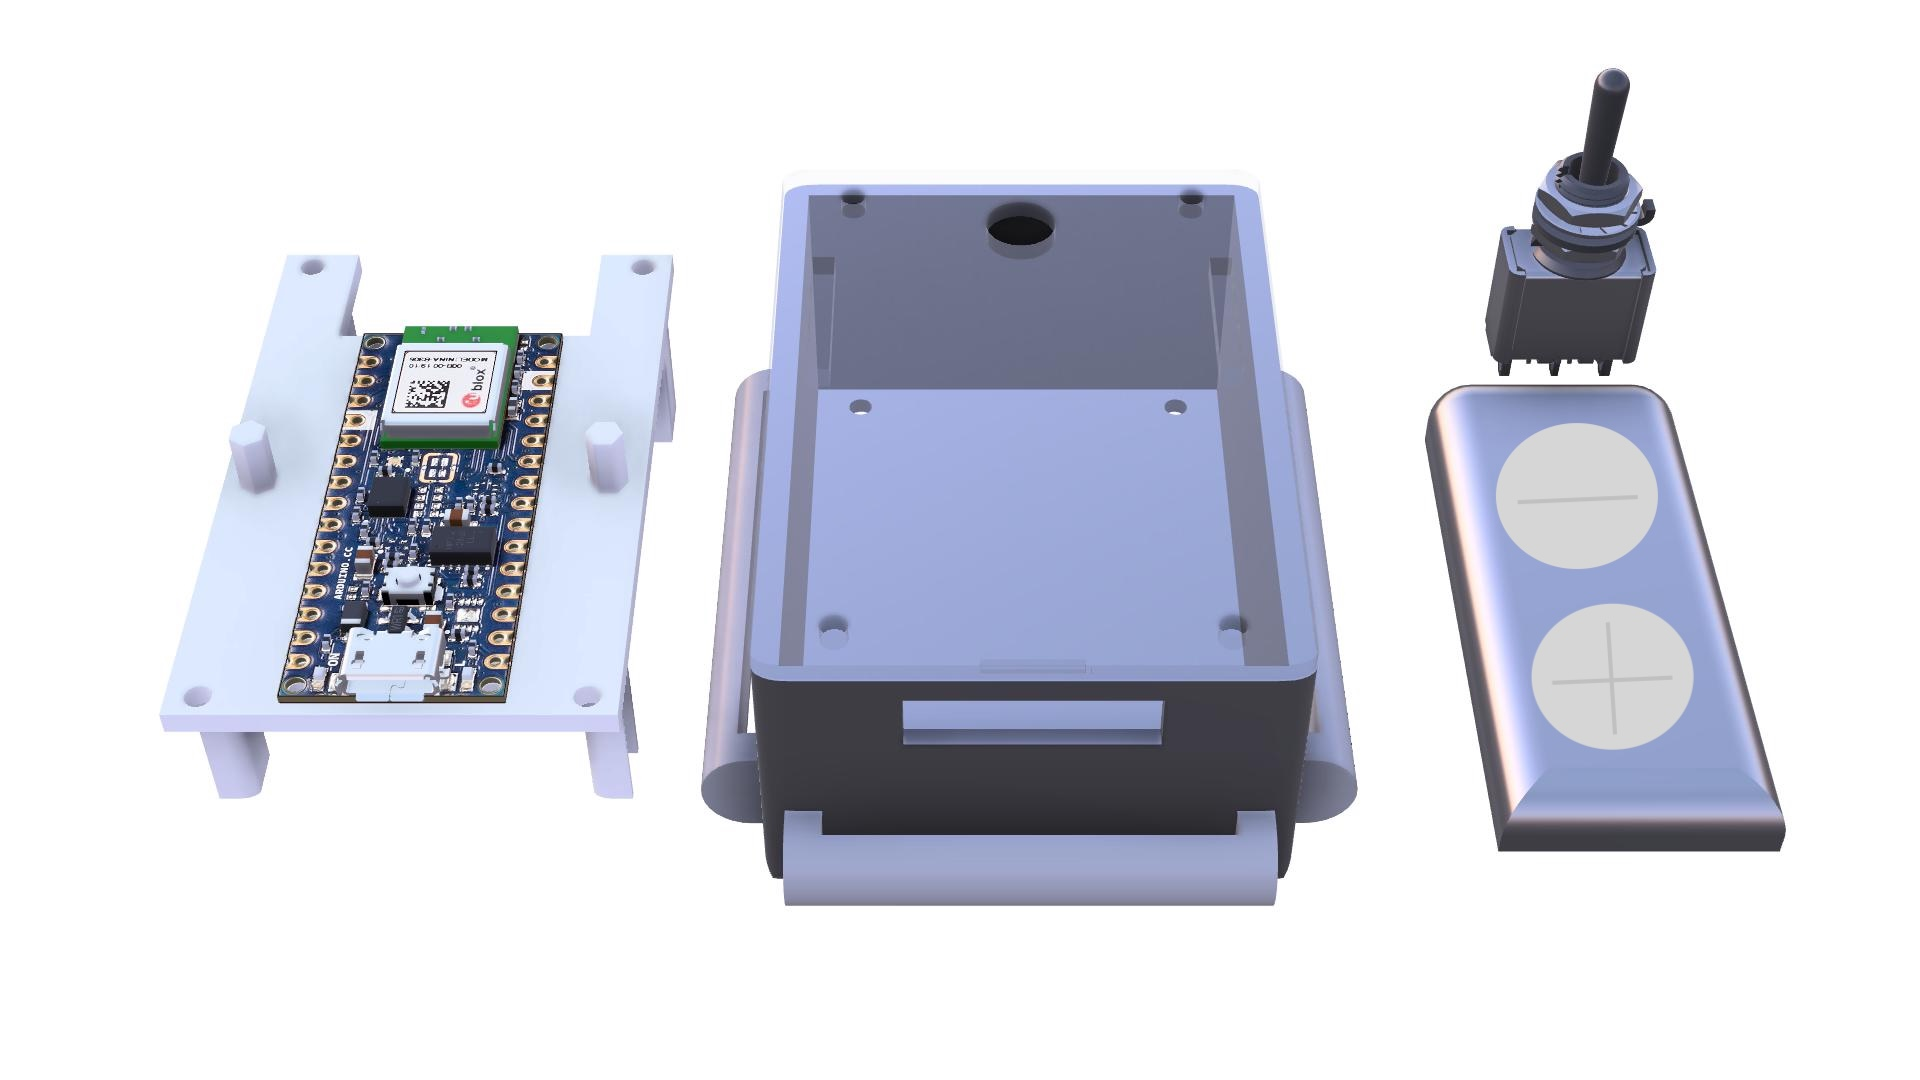
\includegraphics[width=1.1\linewidth]{images/components} % Exploded view
        \end{tikzfigure}
        \textbf{Fig. 2:} Prototype in components.
        }
    }

    \block{Results and Performance}{
        {\Large
        The device successfully:
        \begin{itemize}
            \item Detected gait abnormalities in real-time with high accuracy.
            \item Operated efficiently with a reliable energy source and design.
            \item Demonstrated adaptability to varying gait patterns using machine learning models.
        \end{itemize}
        }
    }

    \block{Future Work}{
        {\Large
        \textbf{Future Directions:}
        \begin{itemize}
            \item Extend detection to other mobility disorders.
            \item Enhance hardware for improved usability.
            \item Incorporate cloud-based analysis for long-term monitoring.
        \end{itemize}
        }
    }

    \block{Conclusion}{
        {\Large
        By integrating wearable technology with machine learning, this project provides a cost-effective and practical tool for real-time gait monitoring. The device empowers patients and healthcare providers alike by offering early detection and actionable insights. With further refinements, it has the potential to become a critical tool in addressing Parkinson’s disease and other mobility disorders.
        }
    }
}
\end{columns}

\end{document}
